
Drone à géométrie variable
\textit{Inspiré de la thèse de Valentin RIVIERE,
<< Vers un robot aérien autonome bio­inspiré à morphologie variable >>,
Thèse de doctorat en Sciences du Mouvement Humain, Aix-­Marseille, 2019}

\section*{Présentation générale}


Ce sujet porte sur la conception d’un drone quadrirotor bio­inspiré, développé à l’institut des
sciences du mouvement. Ce drone s’inspire de l’oiseau et possède la capacité de se replier
en vol afin de diminuer son envergure (\autoref{fig_ccinppsi2022:01} et \autoref{fig_ccinppsi2022:02}).

En fin de repliement, les bras supportant les moteurs et hélices s’alignent le long du corps
du drone pour éviter que les hélices ne touchent les bords de l’ouverture.

Cette particularité est intéressante pour des problématiques d’évitement d’obstacles dans
des milieux encombrés. Le drone est de plus pourvu d’un algorithme d’estimation de taille
d’obstacles en vol grâce à une perception visuelle monoculaire. Cet algorithme permet de
rendre le drone plus autonome pour éviter les collisions avec son environnement et actionner
son système de changement de forme si cela est nécessaire.

Tout cet ensemble constitue la plateforme Quadmorphing.


\begin{minipage}[c]{.48\linewidth}
\begin{figure}[H]
\centering
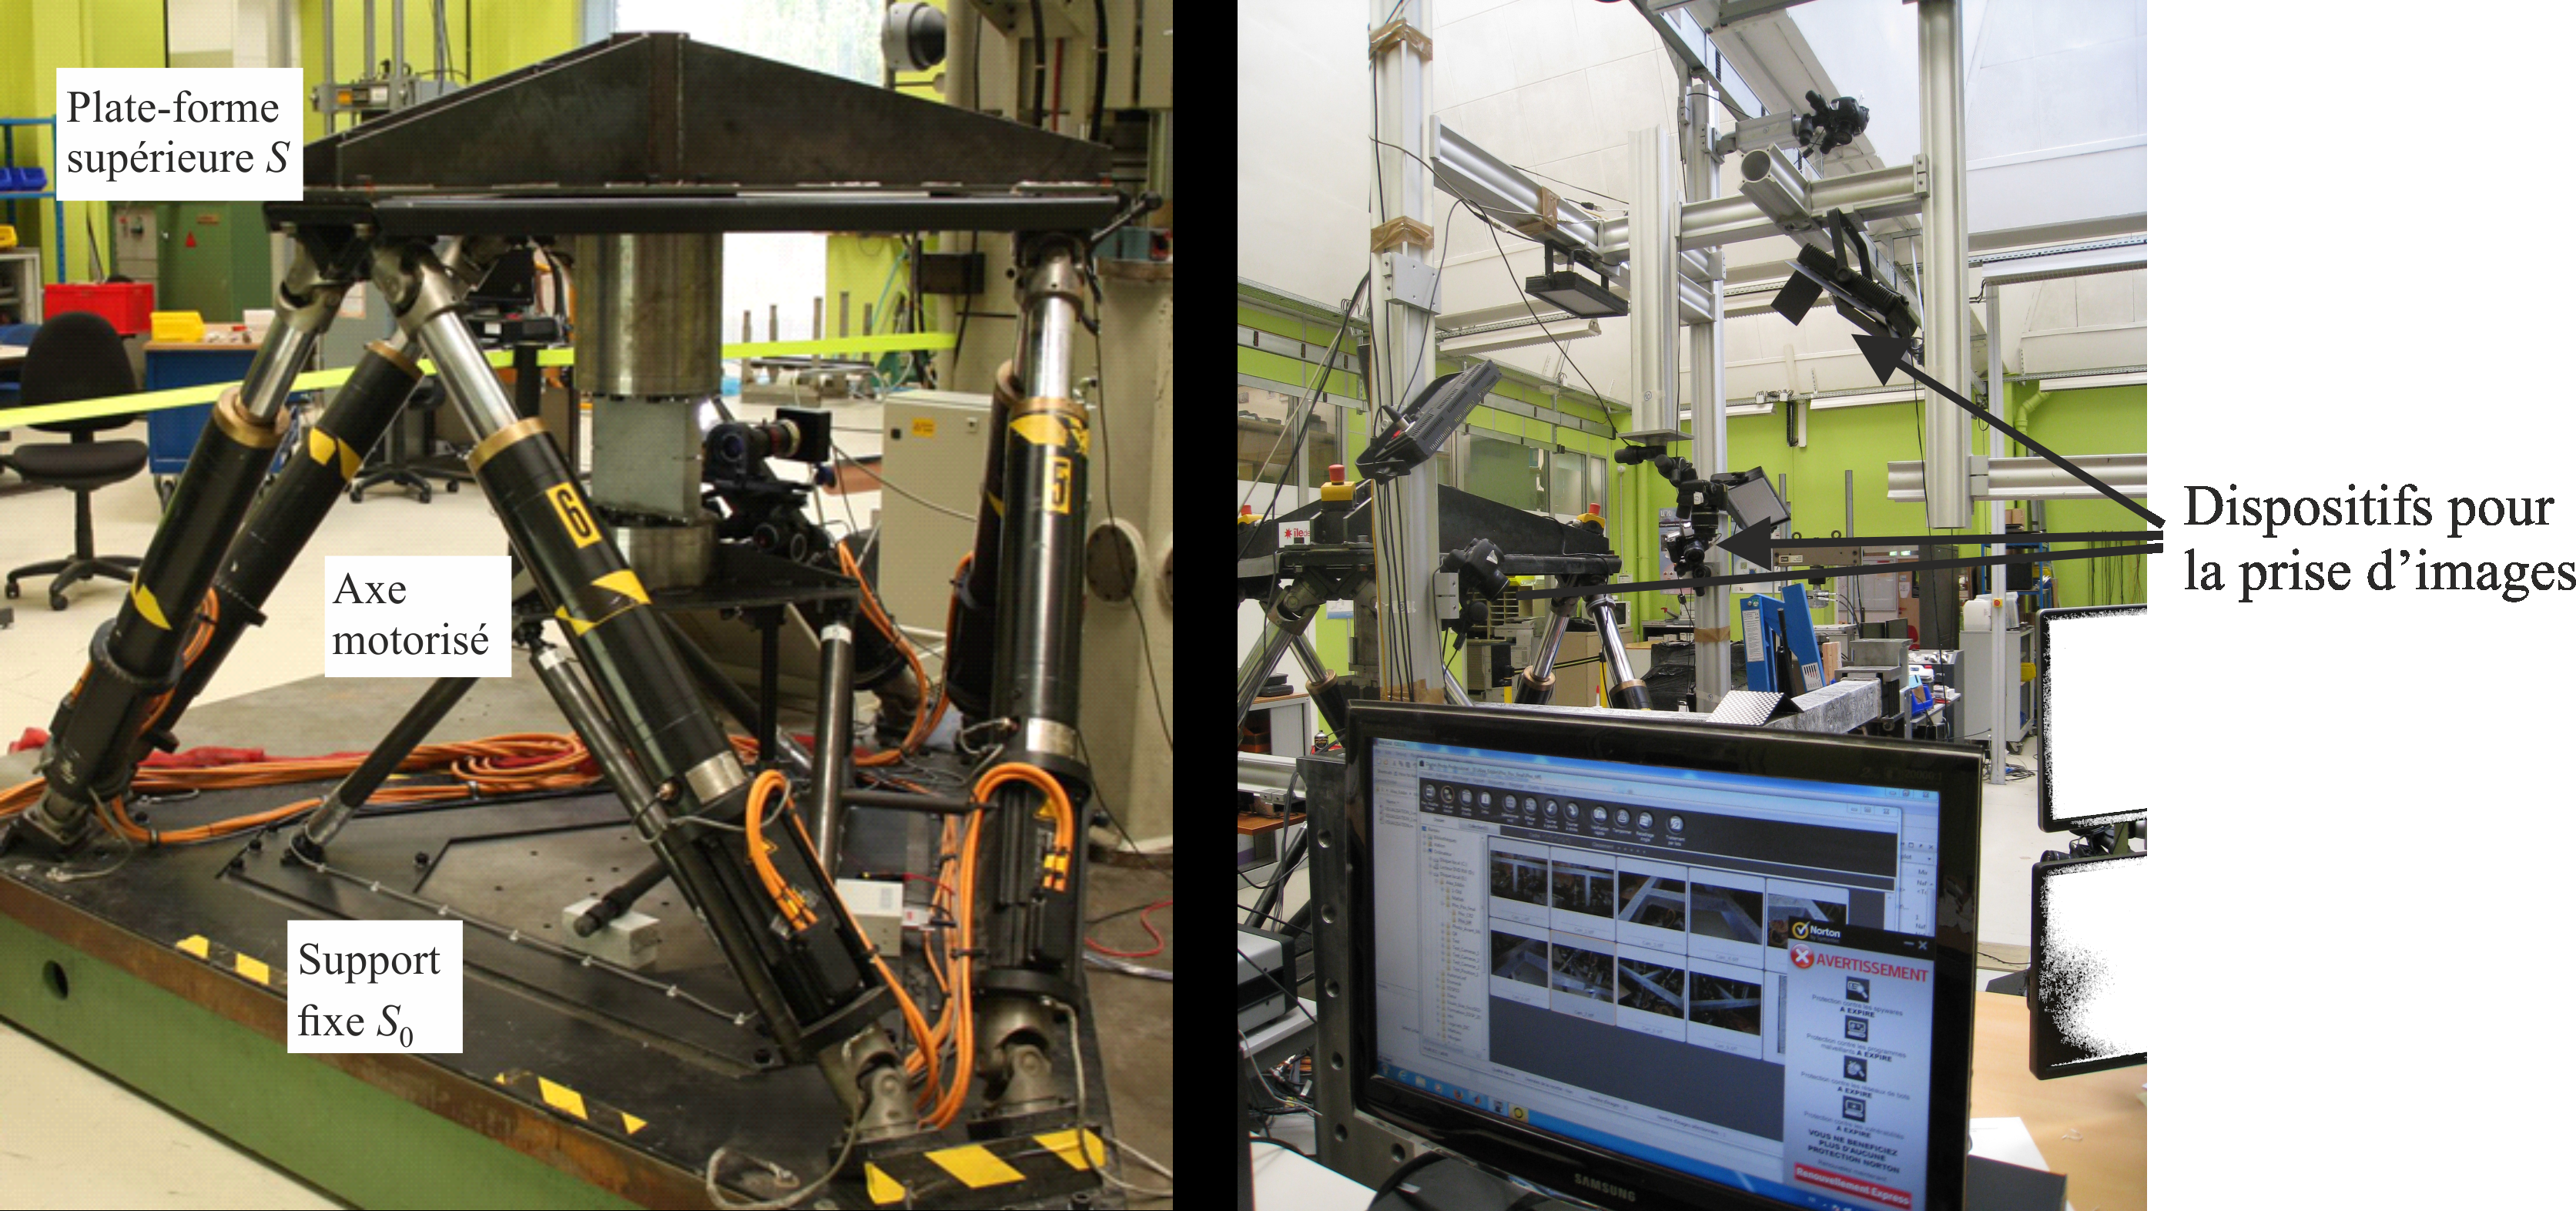
\includegraphics[width=.8\linewidth]{fig_01}
\caption{\label{fig_ccinppsi2022:01} L’oiseau s’adapte au passage
plus étroit en modifiant son envergure}
\end{figure}
\end{minipage}\hfill
\begin{minipage}[c]{.48\linewidth}
\begin{figure}[H]
\centering
\includegraphics[width=.8\linewidth]{fig_02}
\caption{\label{fig_ccinppsi2022:02} Vue CAO de la plateforme QuadMorphing passant à travers une ouverture}
\end{figure}
\end{minipage}

\begin{obj}
L'objectif de cette étude est de concevoir et valider les solutions technologiques retenues
pour la plateforme QuadMorphing permettant le passage d’ouverture en vol. Le diagramme
partiel des exigences liées à cette étude est donné en \autoref{fig_ccinppsi2022:21} de l’annexe 1.
La démarche proposée est définie ci­-après :
\begin{itemize}
\item ­\autoref{sec:01} --­ influence des mouvements des bras du drone sur son comportement;
\item ­\autoref{sec:02} --­ choix d’un mécanisme de modification de l’envergure;
\item ­\autoref{sec:03} --­ analyse simplifiée de l’asservissement en roulis du drone.
\end{itemize}
\end{obj}
